\section{Grundlagen des Buck-Konverters in DC-DC-Wandlern}

\subsection{Hauptkomponenten und Funktionen eines DC-DC-Konverters}

Die Wandlung von Gleichspannung (DC) in eine andere Gleichspannung ist ein kritischer Aspekt in der Elektronik und Energieversorgung. Ein weit verbreitetes Schaltungsdesign, das diese Funktion ausführt, ist der Buck-Konverter. In der Literatur wird dieser als eine Standardmethode für DC-DC-Wandlung beschrieben \cite[p.~66]{wensdesign2022}.



\subsubsection{MOSFET-Transistor}
Der MOSFET-Transistor agiert als elektronischer Schalter, der den Stromfluss in der Schaltung reguliert. Im Vergleich zu alternativen Schaltelementen bietet der MOSFET eine signifikante Effizienzsteigerung durch minimale Leistungsverluste. Dies wird durch Phänomene wie Trägermobilität und die damit verbundene Widerstandsfähigkeit gegenüber thermischen Ausfällen ermöglicht \cite[p.~29]{choi2013pulsewidth}.

\subsubsection{Induktivität (Spule)}
Die Induktivität dient der temporären Energiespeicherung in Form eines magnetischen Feldes, das beim Stromfluss durch die Spule generiert wird. Dies ist insbesondere relevant in Anwendungen wie Solenoid-Antriebsschaltungen, wo die Induktivität als Energiespeicher und -überträger fungiert \cite[p.~54]{choi2013pulsewidth}.

\subsubsection{Diode}
Die Diode ist so ausgerichtet, dass sie den Strom nur in einer Richtung passieren lässt. Dies ist insbesondere wichtig, wenn der MOSFET-Transistor deaktiviert ist. Als passive Schalter werden oftmals schnelle Erholungsdioden oder Schottky-Dioden aufgrund ihrer exzellenten Schalteigenschaften verwendet \cite[p.~29]{choi2013pulsewidth}.

\subsubsection{Kondensator}
Der Kondensator dient der Glättung der Ausgangsspannung und speichert Energie für die Last. Er spielt eine wichtige Rolle in der Dynamik der Schaltung und ermöglicht eine stabilere Energieversorgung \cite[p.~54]{Kularatna2012}.
\subsubsection{Regelung und Anwendungen}

In der Praxis werden Buck-Konverter oft von einer nicht-idealen Spannungsquelle gespeist und müssen daher unter variablen Eingangsspannungen und Lastströmen arbeiten \cite[p.~124,120,113]{choi2013pulsewidth}.. Daher ist eine geschlossene Regelungsschleife erforderlich, um eine konstante Ausgangsspannung sicherzustellen.

Buck-Konverter finden eine breite Anwendung in verschiedenen elektronischen Geräten und Systemen. Ihr hoher Wirkungsgrad, der in der Regel zwischen 75\% und 98\% liegt, macht sie besonders attraktiv.


\begin{figure}[htbp]
    \centering
    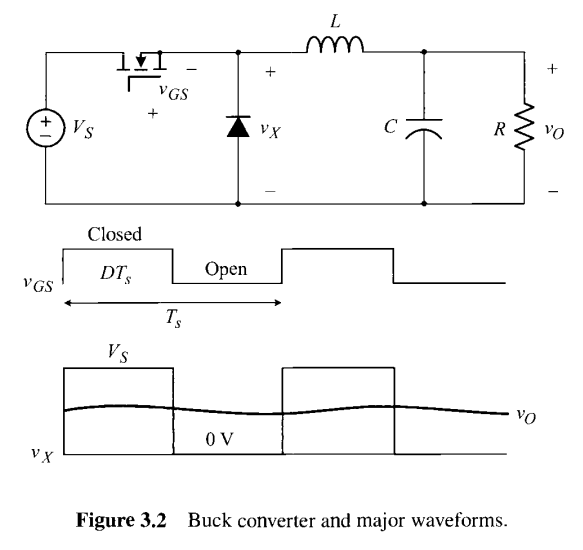
\includegraphics[width=0.4\linewidth]{2Grundlagen/111DCDC.png}
    \caption{Schematische Darstellung eines DC-DC Konverters. Quelle: \cite[Seite 88]{choi2013pulsewidth}}
    \label{fig:dcdc_converter}
\end{figure}



